\documentclass{amsart}
\usepackage[usefamily=sage]{pythontex} 
\usepackage{float}
\usepackage{tikz}
\usetikzlibrary{calc}
\usepackage[utf8]{inputenc}
\usepackage[most]{tcolorbox}
\usepackage[margin = 2cm]{geometry}

\newtheorem{ejer}{Ejercicio}
\def\r{\mathbb{R}}
\title{Tarea 08. Giros en el Plano \\ AMD 2023-24}

\begin{document}
\maketitle

\begin{ejer}
Construye la bandera de Chile con la especificaciones indicadas el el siguiente gráfico:

\begin{figure}[H]
\centering
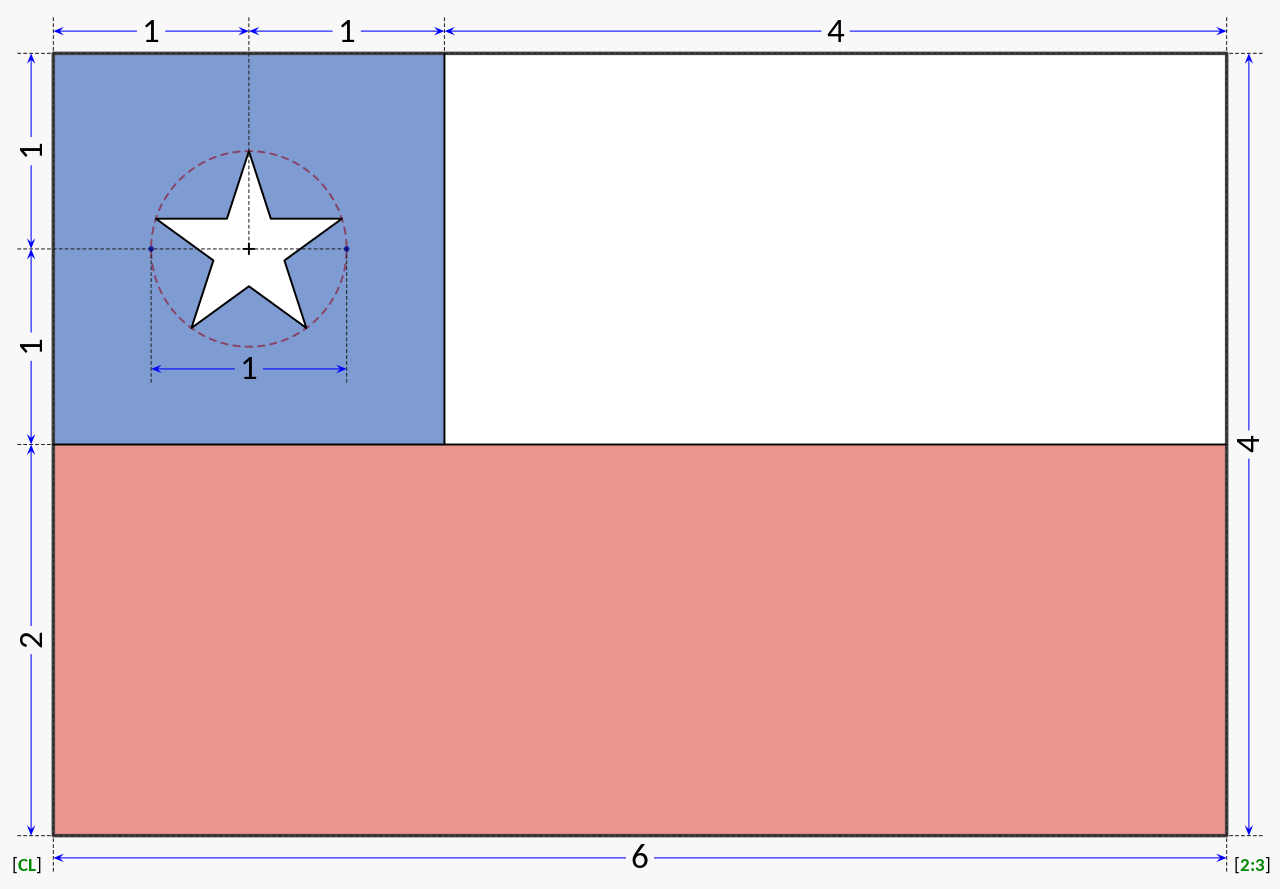
\includegraphics[width = 12cm]{Chile.png}
%(Fuente: \url{https://en.wikipedia.org/wiki/Flag_of_Chile#/media/File:Flag_of_Chile_(construction_sheet).svg})
\end{figure}
\end{ejer}

{\it Solución:}

% Escribe tu solución para el ejercicio 4



\end{document}
